
% CHAPTER 1

\chapter{INTRODUCTION}
\label{chp:introduction}

In this thesis work, it is aimed to create a novel method for formation control of a swarm which consists of heterogenous mobile robots. The term of swarm represents a large group of locally interacting individuals with common goals[4]. 

Self organizing swarm researches and its applications are generally inspired by the biological systems in the nature. 
The behaviours of these biological systems were considered mysterious and strange for a long time, but in recent researches show that individuals don't need any sophisticated knowledge or top level functionalities to produce such complex tasks[2] . These biological systems (e.g. colony of ants) have simple behaviours but they can accomplish very complicated collective tasks in the nature which are impossible with their own individual capabilities. Beni [1] describes this collaboration of members as follows:

The group of robots is not just a group. It has some special characteristics, which are found in swarms of insects, that is, decentralised control, lack of synchronisation, simple and (quasi) identical members.

It is obvious that such a collective behaviour of these swarms has more power and efficiency than the sum of the individual capabilities of the members. 

General aspects of the swarm robotics systems are the simplicity of individuals, restricted sensing and communication capabilities, achieving tasks mutually, robustness and decentralized control capability[6].


Swarm robotics has been studied to produce different collective behaviors to solve tasks such as as aggregation , pattern formation , self-assembly and morphogenesis , object clustering, assembling and construction , collective search$\&$rescue and exploration , coordinated motion , collective transportation , self-deployment , foraging and others[5]. Dorigo and Trianni[7] are studied on controllers for aggregation of coordinated motion of the identical mobile robots called swarm-bots.  Hou, S.P., C.C. Cheah, and J.J.E. Slotine is focused on controlling of a swarm within a dynamically changing formation[8]. Ganesh and Lisa introduced two new strategies for collective search and exploration of fields with swarm intelligence[9]. Chaimowicz and Campos proposed a new methodology which is based on a dynamic role assignment mechanism in which the robots cooperate with each other and they demonstrate this method in a cooperative transportation task[10].  Campo and Gutierrez is studied on collective foraging task and they propose a method for path selection to optimize the profits of the swarm[11].

There are lots of studies related with different problems in swarm robotics literature as discussed briefly. In this thesis project, we are focused on dynamic pattern formation control of swarms consist of heterogeneous robots.


\section{Problem Definition}
In this thesis work, the main idea is to propose a complete design solution to a dynamically changing formation system, including a local positioning system and formation control system. The swarm which is used in this formation system is assumed to be composed of heterogenous agents which have different functionalities and physical properties. The formation shape is expected to be closed contours which cannot be identified with analytical expressions and these shapes will be changing dynamically with a continuous manner. 

Formation control system is heavily depend on the position data of individual agents in the environment. Since it is expected to have high number of agents in the environment due to the nature of a swarm, the agents are assumed to have simple structures with low capabilities including certain types of sensors. On the other hand, for indoor applications it will not be possible to use satellite dependent positioning systems on agents. Even if a positioning solution depending on different methods including visual feedback(by image processing), RSS(received signal strength) etc. is available for an indoor application, it is not possible to implement this solution for each single agent in the environment due to the increasing complexity and the costs by the number of agents. As a result of these constraints, it is required to implement a localization solution for the agents to provide the corrected positions in the workspace to be used by the formation control system. This localization process have to correct the position data of the agents with the determined process period and within an maximum error bound which will be determined by the requirements of the formation control problem. 

Formation control system have to provide a solution to the coverage of a dynamically changing formation shape by the agents in the swarm. Desired formation shapes will not be simple geometrical shapes like circles, triangles etc.  Heterogenous agents with different shapes have to cover the instant formation shape homogenously as possible as. The total displacements of the agents while travelling towards the desired formation have to be minimized. In other words, agents have to adapt the new formation shape with minimum possible movement. On the other hand, collision avoidance with the obstacles in the workspace and with the other agents has to be provided while achieving different types of formation tasks. Each agent must execute its own controller-decision making algorithms in a decentralized manner. 
\section{Motivation}

The formation control problem can be defined as collaboration of an agents' group to maintain a formation with a certain shape [12]. It focuses on leading the individual agents of a swarm to perform  collective tasks including shape generation and formation reconfiguration while traversing a trajectory by providing collision avoidance simultaneosuly. These kind of tasks are achieved with a large group of small and simple robots  that can cooperate with each other. Formation control of multi agent systems  is an actively growing research field.\newline 

Swarms which are used in formation control systems, can be composed of homogenous or heterogenous agents according to the requirements of the problem. The usage of the homogenous agents increases the total energy and the coverage of the system in the environment. This kind of a swarm has an increased redundancy and is capable of resuming the current task in case of failures of some of the agents during mission. On the other hand, a swarm composed of heterogeonus agents holds the different capabilities of the agents. This kind of a system can be used in tasks which requires different functionalities has to be performed individually or simultaneously.\newline

In real world applications there may be need for different  functionalities to achieve some specific tasks. If this is the case, one solution may be to design a sophisticated robot which includes all required capabilities for this task. In this scenario, this robot will be the single point of failure in the system and if robustness is a  vital feature for this solution, some redundant robots have to be added to the system. It is clear that the design of such an advanced robot and hold its redundant backups in the system will increase the cost of the solution. In swarm robotics concept, one of the approaches related with the usage of the heterogenous agents is to gather some different types of simple mobile robots which have their own specific functionalities to achieve a collective task rather than designing an advanced robot for the solution. With this approach, the robustness of the system is increased, costs are reduced down and the reusability of the individual members of the swarm for other tasks is provided.  A project named Swarmanoid which is funded by European Commission, has an objective to implement and control of a novel distributed robotic system. The system is made uo heterogeneous, dynamically connected, small autonomous robots called,  foot-bots , hand-bots and eye-bots where foot-bots are responsible to transport the required materials(including other types of robots) to a specific task area and foot-bots are responsible of operations with their manipulators in and eye-bots are responsible of observations and reconnaissance on the area.

	\begin{figure}[H]
		\caption{A Robot Team Consists of Eyebot, Handbot and Footbot Agents}
		\centering
		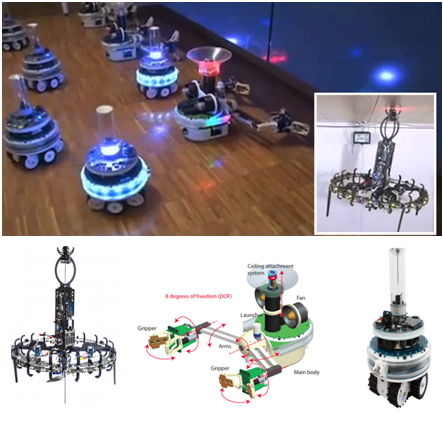
\includegraphics[scale = 1]{eyebot}
	\end{figure} 


A swarm which is composed with same type of homogenous agents can be used to increase the total impact and the energy of an individual agent. This kind of a system can be used in missions like coverage, search and  reconnaissance etc.  Martin and Kilberg have worked on formation control and formation tracking of  microsatellites to achieve continous coverage and improved capability. They also mentioned that small formations will reduce the fuel consumption for propulsion and expand the sensing capabilities of microsatellites[15].

	\begin{figure}[H]
		\caption{Sparse Aperture Formation of Micro Satellites}
		\centering
		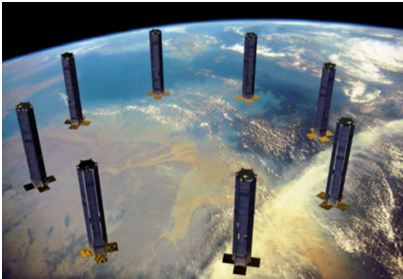
\includegraphics[scale = 1]{Satellite}
	\end{figure} 


Formation control solutions has lots of usage areas such as coverage missions, security patrols and search$\&$rescue in hazardous environments etc.[13]. For missions related with area coverage and reconnaissance, a group of autonomous vehicles may be required to keep in a specified formation [13].  Balch and Arkin presented a behaviour based formation control for multi robot teams which is implemented on a team of robotic scout vehicles manufactured for a DARPA project[14]. 


\begin{figure}[H]
	\caption{A team of four robotic scout vehicles on which formation control techniques implemented}
	\centering
	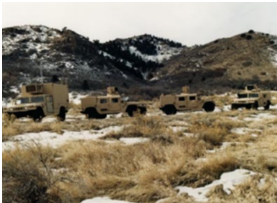
\includegraphics[scale = 1]{scout_robots}
\end{figure} 

There are some hardware implementations to test the related formation control algorithms in real time applications. Since the formation control problem requires lots of agents in a swarm, these works are have a common point of providing agents with minimal costs and sensor capabilities. The Kilobot Project from Harvard university have released their agents with the name of Kilobots and they have teams which are working on different formation control problems with Kilobots.


	\begin{figure}[H]
		\caption{Formation Control with Kilobots}
		\centering
		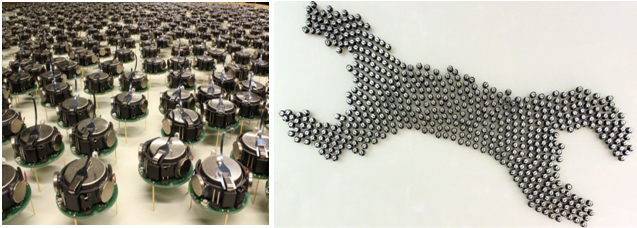
\includegraphics[scale = 1]{kilobot}
	\end{figure} 


These micro robots have a great reusability for different types of formation control problems  and they have biological insprations from the nature in the sense of individual simplicity and power of collective behaviors.

	\begin{figure}[H]
		\caption{A) Swarm Robot Project from Universities of Stuttgart  \\
            			B) Colias Project from University of Lincoln and Tsinghua University in China\\
			            C) Marx bot developed at EPFL \\
            			D)Swarm bots project conducted by  European Commission			}
		\centering
		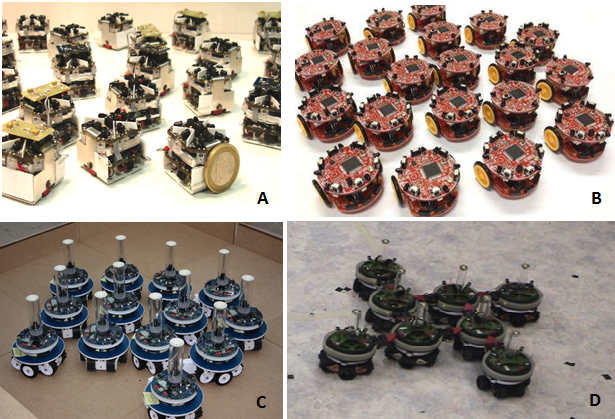
\includegraphics[scale = 1]{mobilerobots}
	\end{figure} 


\section{Objectives}


In this thesis work, our aim is to provide different approaches $\&$ solutions to the requirements in formation control problem.  There are mainly different types of  infrastructures while providing a global solution to the formation control problem like the heterogeneity vs. homogeneity of the agents, communication structures, centralized vs. decentralized structures, swarm control strategies like behavior based and leader-following approaches or virtual structure based approaches. 

In addition to choice of the formation control infrastructures, capabilities of the individual agents provide additional requirements and constraints while designing a formation control system. One of the most important characteristic of an agent in the swarm is its simplicity and limited sensor $\&$ communication capability. This approach results from the idea of achieving collective tasks with lots of simple individuals  and it is based on biological inspirations in nature like colony of ants etc.

In this project the defined requirements and objectives are given as follows;

\subsection{Heterogenous Robots with Different Dynamics}


Agents have different dynamics from each other like different friction surfaces, geometrical structures and functionalities. They have different volumes and masses(not mass point particles) and they may collide with the other ones and the obstacles in the environment. 


	\begin{figure}[H]
		\caption{Heterogenous Agents with Different Physical Properties and Functionalities}
		\centering
		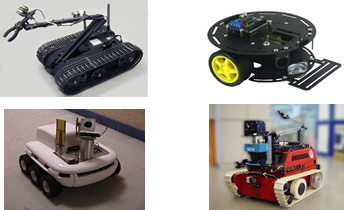
\includegraphics[scale = 1]{heterogenous}
	\end{figure} 
	
	

\subsection{Communication Infrastructure}

Agents in the swarm have limited communication capabilities and can only negotiate with its local neighbors in a narrow line of sight range due to power consumption issues and their weak radio links.

\begin{figure}[H]
	\caption{Radio Links on Agents have a narorw LOS range}
	\centering
	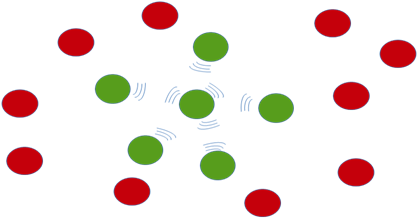
\includegraphics[scale = 1]{narrow_los}
\end{figure} 



a)Communication Topology


Communication topology is a wireless mesh network in which each agent relays data for the network. The network is fully connected and has routing technique where the data is propogated along a route by transporting over the nodes(member agents of the swarm) . 

\begin{figure}[H]
	\caption{Mesh Network Between Agents}
	\centering
	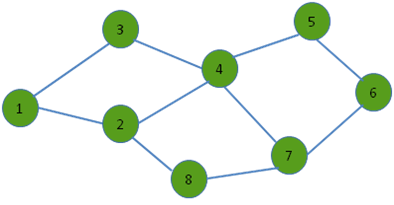
\includegraphics[scale = 1]{mesh}
\end{figure} 

b)Communication Bandwith

Bandwith of the communication between agents is limited and nodes can only transport most critical data like heartbeats, agent IDs, type and position etc. 



\subsection{ Decentralized Decision Making Process}

Centralized formation controller systems implement a single controller  server/root node
to process all the data needed to achieve the desired control objectives. This type of systems achieve superior performance and optimal decisions  but they require high computational power, high communication bandwiths and are not robust due to dependence on a single controller[12]. Decentralized formation controller structures have agents which are completely autonomous and responsible their own individual decisions. In this work, a hybrid centralized/decentralized controller architecture in which there is a central manager which partitions the desired formation shapes into goal states and there are independent agents who make their own choices on these goal states to reach as unaware of the other agents' choices. 


\begin{figure}[H]
	\caption{Agents make their own choices about target goal states}
	\centering
	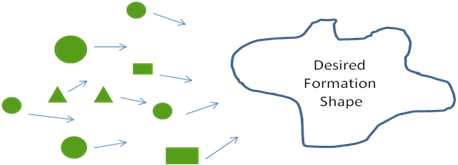
\includegraphics[scale = 1]{decentralized}
\end{figure} 


\subsection{Complex Closed Contours}
Formation shapes will be defined as closed curves with complex shapes and they cannot be identified analytically . On the other hand shapes will be changing dynamically during formation control. 

\begin{figure}[H]
	\caption{Complex and Dynamically Changing Formation Shapes}
	\centering
	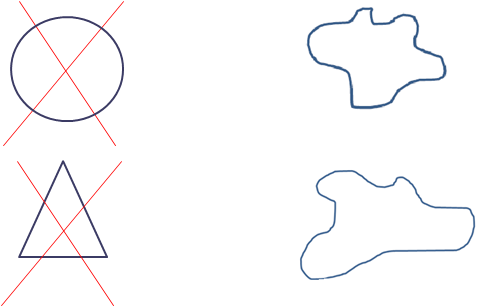
\includegraphics[scale = 1]{complex}
\end{figure} 



\subsection{Simple Agents with Low Sensor Capabilities and Low Computing Powers}


Agents in the swarm are assumed to have low sensor capabilities and weak computing power. This 
condition must be taken into account during the control system design, since individuals do not have a high resolution and sensitive data about their state vectors, and they cannot run high level complex control algorithms.


\section{Goals}

The objectives and the assumptions about the requirements define the goals of this thesis project. The goals of the project are listed in the following section.

1. Agents have to propogate their position and velocity states with the help of inertial measurements.This process is handled with a Kalman estimator which takes the translational accelaration data as an input to the observer model .The translational acceleration data is calculated with the help of AHRS system composed by 3 axis accelerometers, gyroscopes and magnetometers. 

2. Agents have to update$\&$adjust the position data with the help of agents which have positioning sensors(position beacons) by local trilaterations.This position data is used in the internal estimator systems as external measurements to correct the drifts caused by propogation error of translational accelerations.  The ordering for this trilateration process have to determined appropriately to minimize the error on calculated position data of agents which are far away from the position beacons.

3. Agents have to update their route tables to create a communication backbone with the mesh network topology. Since agents are assumed to have low range$\&$bandwith radio links, the propogation of a data between each agent in the swarm will be handled over this mesh network. 

4. Agents have to determine the goal states in the desired complex formation shape to cover with the help of a central server. Desired formation shape will be partitioned into potential goal states assigned to different types of agents. Performance analysis on proposed shape partitioning methods have to be done with some different criterias. 

5. Assignment of the agents to their target goal states should be handled to minimize the total displacement of the agents while travelling towards the desired formation shape. 

6. Simulations should be performed to compare the efficiency of different methods proposed in this thesis work   Differnt types of agents have to be represented with different dynamical and physical models during simulations.

7. Hardware demonstrations should be performed to illustrate the applicability of the proposed solution in real time systems. These applications may not contain the full implementation of the proposed system, but they must demonstrate the proof of concept(POC) environment. 


\section{Methodology}

During the first part of the project, a local positioning system(LPS) is designed. In this system, agents which does not have position sensors propogate their position and velocity states with their inertial measurements. Due to the bias and drift errors on this solution a position update$\&$adjust process is handled on 0.1Hz frequency with the help of position beacons which are agents with position sensors on board in the swarm.. During the update phase of the solution route tables for individual agents are determined with the help of Graph Theory based Destination-Sequenced Distance Vector Routing Protocol (DSDV) algorithms. This process provides the clusters around position beacons and provides rank information for the agents which are in same clusters. Position measurements are handled with local trilateration process in turn with the rank values for every agent around each clusters after the establishment of route tables. A Kalman estimator system is designed to fuse these propogation and update phases of the solution.

Formation controller system is designed with two novel methods based on artificial potential force methods and advancing front local reconnection method. Desired complex formation shapes are partitioned into goal states according to the heterogenous agents in the swarm for both of these two methods. Decision process of the agents about their target goal states to optimize the overall utility of the swarm is implemented with the help of Visibility Graphs and Hungarian algorithms. Internal velocity controllers for individual agents to reach the desired target goal states by providing obstacle avoidance, are implemented with a full state feedback method by regulating the dynamical system with the gains optimized by Linear Quadratic Regulators (LQR).


\section{Contribution of Thesis}

The main contributions of thesis are:

1. Designing a local positioning system(LPS) based on local trilaterations to provide a high accuracy position data to the agents which do not have a specific position sensors on their boards.

2. Implementing a wireless mesh network between agents in the swarm and design a communication infrastructure and related routing algorithms to exchange the local data globally in the network

3. Partitioning the complex formation shapes into goal states to cover the whole formation homogenously with the different types of heterogenous agents.

4. Designing and implement the rules$\&$algorithms for the decision process of the individual agents about the goal states to reach.

5. Designing a simulation environment to test the proposals and algorithms of this thesis work

6. Designing a simple demonstrative hardware application.


\section{Outline of the Thesis}
This thesis work is organized into 5 main sections .Chapter 1 introduces the main theme and the potential areas of the usage of formation control, while specifying our motivation and the requirements$\&$problems to meet$\&$solve related with the topic.

Chapter 2 gives literature reviews about the related works and basic mathematical background on the methods used in this paper.

Chapter 3 introduces the methods and solutions used in two different parts of the problem; local positioning system and formation conroller system. In this chapter, routing algorithms and mathematical aspects of the trilateration process is introduced. Methods$\&$algorithms used for formation control is discussed in details.

Chapter 4 provides simulation analysis on the local positioning system and gives mutual evaluations of the performances of different methods used in formation control system.

Chapter 5 provides the details of hardware implementations and the experimental results.

Chapter 6 concludes the thesis and defines the future works related with the thesis.